% -*- root: ../main.tex -*-
\subsection{Representing a program in logic}

\subsubsection{Preliminaries (Notation, definition)}

One can consider a program as a series of state changes. There are some variables, we execute one line of the program and some of those variables changes and some others don't. Thus, we can consider any program as a graph of states with some ways. For example, lets take a very simple program:

\[
	\begin{array}{l@{\hspace{0.3em}}c@{\hspace{1em}}l}
	\hline
		l_1 & : & \mathtt{x := -2} \\
		l_2 & : & \mathtt{\textbf{if } (x<0)} \\
		l_3 & : & \mathtt{\;\;x = 2x} \\
		l_4 & : & \mathtt{\textbf{...}}\\
	\hline
	\end{array}
\]
\label{simple:example}

This simple program doesn't do anything interesting, but it is useful to illustrate. This is the directed graph of states.

\begin{figure}[hbtp]
\centering
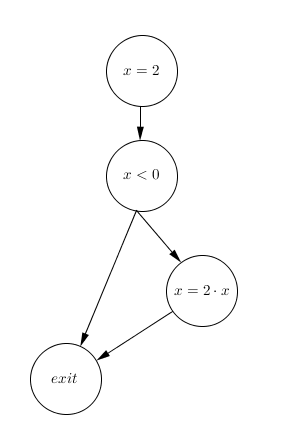
\includegraphics[scale=0.6]{graphics/simpleExample.png}
\caption{Directed graph of the program \ref{simple:example}}
\end{figure}


In the execution of this program, it is not possible to execute line 3 just after line 1 skipping line 2. We need to go line by line, respecting the execution flow. 
This is represented by the variable \pc (\concept{Program\IS counter}). This variable indicates the line to execute next.

So the state of the program at the begining is 

\[ \pc = 1\]

This formula give all the information we have of the execution state. We know the \pc and the state and value of all variables (there are no more variables than \pc).

Now we need to define the step. 
%
How can we represent the execution of a line.
%
We need to use \concept{post-state} variables. 
%
We define the prime version of any variable to refer that same variable after the execution of the line (transition). 
%
Going back to the example, we have:

\[
\pc = 1 \andcond \pc'=2 \andcond x'=2 
\]

We have a post-state program counter ($\pc'=2$) and some post-state variables. 
%
As the execution of the assignment the variable $x$ takes a value (independently of the value in the pre-state), then $x'=2$ (regardless what value $x$ has). 

The next step could be
\[
\pc = 2 \andcond x'=x \andcond 	\pc'=?
\]

Where \? depends on the validity of the \textit{if} condition. 

This steps we have illustrated are called transition relations.

\begin{defn}[Transition relation]
A transition relation is the formula that define the step from one step of the program to another.  
\end{defn}

With this simple example, we have shown what a program counter and what a transition relation are. Now we can define the possible instructions a program may have.\footnote{We have just took the set of instructions the programs we are going to proof have.}


\todo{heap, cell}

\subsubsection{Possible instructions}
As we are going to work with programs used by more than one thread, we need one program counter for each thread executing. 
%
We parametrize the program counter. 
%
This is, defining the \textbf{program counter} as a \textbf{function} that given a thread, returns its program counter. 
%
We could have define as one variable per thread, but it would be equivalent. 

For this definitions we use the letter $T$ to refer a particular thread.

\begin{description}
\item [Assignments:]
		The transition relation for a variable assignment consists of the 
		update of the program counter for the running thread and the 
		corresponding modification to the variable being assigned.
\[
\begin{array}[t]{p{8em}@{\hspace{6em}}p{\longtablesize}}
	\hline
	Statement & Transition relation \\ \hline\hline
	$\begin{array}[t]{l@{\hspace{0.3em}}c@{\hspace{1em}}l}
		l_1 & : & \mathtt{v := 2} \\
		l_2 & : & \mathtt{\cdots}
	\end{array}$
	&
	$\begin{array}[t]{ll}
		 \pc(T) = l_1 \andcond
		 \pc'(T) = l_2 \andcond
		 \mathtt{v}' = 2
	 \end{array}$ \\ 
	 \hline
\end{array}
\]

	\item [Pointer access:]
		Cell fields are accessible through the pointer operator \pointsto.
%
		There are two possible scenarios for the use of pointers, depending on 
		whether the statement accesses or modifies a cell field.
%
		We present now the semantics for both cases.
%
		The first case corresponds to the access of a cell field through an 
		address pointer.
%


\[
\begin{array}[t]{p{8em}@{\hspace{6em}}p{\longtablesize}}
	\hline
	Statement & Transition relation \\ \hline\hline
	$\begin{array}[t]{l@{\hspace{0.3em}}c@{\hspace{1em}}l}
		\ell_1 & : & \mathtt{v := a \pointsto field} \\ \\
		\ell_2 & : & \mathtt{\cdots}
	\end{array}$
	&
	$\begin{array}[t]{ll}
		 \pc(T) = \ell_1 \andcond
		 \pc'(T) = \ell_2 \andcond \\
		 \mathtt{v}' = \heap[\mathtt{a}].\mathtt{field}
	 \end{array}$ \\
	 \hline
\end{array}
\]

		The second case corresponds to the modification of a cell field using 
		an address pointer.
%
		Note how, in the second case, all cells (except the one pointed by 
		$\mathtt{b}$) remain unchanged.
%
		Also, all fields of the cell pointed by $\mathtt{b}$ remain unmodified 
		except for $\mathtt{field_n}$.

\[
\begin{array}[t]{p{8em}@{\hspace{6em}}p{\longtablesize}}
				\hline
				Statement & Transition relation \\ \hline\hline
				$\begin{array}[t]{l@{\hspace{0.3em}}c@{\hspace{1em}}l}
					\ell_1 & : & \mathtt{b \pointsto field_n := a} \\ \\ \\ \\
					\ell_2 & : & \mathtt{\cdots}
				\end{array}$
				&
				$\begin{array}[t]{ll}
					\pc(T) = \ell_1 \andcond \pc'(T) = \ell_2 & \andcond \\
					\heap' = \heap \{ \mathtt{b} \leftarrow c \} & \andcond \\
					c.\mathtt{field_n} = \mathtt{a} & \andcond \\
					\bigwedge\limits_{i \neq \mathtt{n}} c.\mathtt{field}_i = 
					\heap[\mathtt{b}].\mathtt{field}_i
				\end{array}$\\ \hline
	\end{array}
\]
	\item [No operation:]
		The no operation statement performs no change at all except from 
		updating the program counter of the executing thread.

\[
\begin{array}[t]{p{8em}@{\hspace{6em}}p{\longtablesize}}
	\hline
	Statement & Transition relation \\ \hline\hline
	$\begin{array}[t]{l@{\hspace{0.3em}}c@{\hspace{1em}}l}
		\ell_1 & : & \mathtt{\SkipStm} \\
		\ell_2 & : & \mathtt{\cdots}
	\end{array}$
	&
	$\begin{array}[t]{ll}
		 \pc(T) = \ell_1 \andcond
		 \pc'(T) = \ell_2
	 \end{array}$ \\ \hline
\end{array}
\]	

	\item [Conditionals:]
		We present now the two possible kinds of conditional statements in 
		SPL.
%
		In the first case, if condition $c$ does not hold, the execution 
		proceeds from the statement following the end of the conditional.

		\[
        \begin{array}[t]{p{8em}@{\hspace{6em}}p{\longtablesize}}
				\hline
				Statement & Transition relation \\ \hline\hline
				$\begin{array}[t]{l@{\hspace{0.3em}}c@{\hspace{1em}}l}
					\ell_1 & : & \mathtt{\textbf{if } c \textbf{ then }} \\ \\
					\ell_2 & : & \mathtt{\cdots} \\
						&& \mathtt{\vdots} \\
					\ell_n & : & \mathtt{\textbf{end if}} \\
					\ell_{n+1} & : & \mathtt{\cdots}
				\end{array}$
				&
				$\begin{array}[t]{ll}
					(\pc(T) = \ell_1 \andcond \;\;\mathtt{c} \andcond \pc'(T) = \ell_2) \; \Or \\
					(\pc(T) = \ell_1 \andcond \lnot \mathtt{c} \andcond \pc'(T) = \ell_{n+1})
				 \end{array}$ \\ \hline
			 \end{array}
		 \]

		In the second case, if condition $c$ does not hold, the execution 
		continues at the first statement in the \textbf{else} section of the 
		conditional statement.

		\[
				\begin{array}[t]{p{8em}@{\hspace{6em}}p{\longtablesize}}
				\hline
				Statement & Transition relation \\ \hline\hline
				$\begin{array}[t]{l@{\hspace{0.3em}}c@{\hspace{1em}}l}
					\ell_1 & : & \mathtt{\textbf{if } c \textbf{ then }} \\ \\
					\ell_2 & : & \mathtt{\cdots} \\
					\mathtt{\vdots} \\
					\ell_n & : & \mathtt{\textbf{else}} \\
					\ell_{n+1} & : & \mathtt{\cdots} \\
					\mathtt{\vdots} \\
					\ell_m & : & \mathtt{\textbf{end if}} \\
					\ell_{m+1} & : & \mathtt{\cdots}
				\end{array}$
				&
				$\begin{array}[t]{ll}
					(\pc(T) = \ell_1 \andcond \;\;\mathtt{c} \andcond \pc'(T) = \ell_2) \; \Or \\
					(\pc(T) = \ell_1 \andcond \lnot \mathtt{c} \andcond \pc'(T) = \ell_{n+1})
						& \text{for line } \ell_1 \\ \\ \phantom{\vdots} \\

						\pc(T) = \ell_n \andcond \pc'(T) = \ell_{m+1} & \text{for line } \ell_n
				 \end{array}$ \\ \hline
			\end{array}
		\]

	\item [Loops:]
		We consider the only loop statement available in SPL which executes 
	the statements in the body as long as the loop condition holds.

		\[
				\begin{array}[t]{p{8em}@{\hspace{6em}}p{\longtablesize}}
				\hline
				Statement & Transition relation \\ \hline\hline
				$\begin{array}[t]{l@{\hspace{0.3em}}c@{\hspace{1em}}l}
					\ell_1 & : & \mathtt{\textbf{while } c \textbf{ do }} \\
					\ell_2 & : & \mathtt{\cdots} \\
					\mathtt{\vdots} \\
					\ell_n & : & \mathtt{\textbf{end while}} \\
					\ell_{n+1} & : & \mathtt{\cdots}
				\end{array}$
				&
				$\begin{array}[t]{ll}
						(\pc(T) = \ell_1 \andcond \;\;\texttt{c} \andcond \pc'(T) = \ell_2) \; 
						\Or \\
						(\pc(T) = \ell_1 \andcond \lnot \texttt{c} \andcond \pc'(T) = 
					\ell_{n+1})
					& \text{for line $\ell_1$} \\ \\
					\pc(T) = \ell_n \andcond \pc'(T) = \ell_1 &
						\text{for line $\ell_n$}
				 \end{array}$ \\ \hline
			 \end{array}
		\]

			\item [Non deterministic choice:]
		The transition relation for the non-deterministic choice statement can 
		be expressed as follows:

		\[
			\begin{array}[t]{p{8em}@{\hspace{6em}}p{\longtablesize}}
				\hline
				Statement & Transition relation \\ \hline\hline
				$\begin{array}[t]{l@{\hspace{0.3em}}c@{\hspace{1em}}l}
					\ell_1 & : & \mathtt{\Nondet} \\
					\ell_2 & : & \mathtt{\;\;\;\;\;\; \cdots} \\
					\ell_3 & : & \mathtt{\textbf{or } \; \cdots} \\
					\mathtt{\vdots} \\
					\ell_n & : & \mathtt{\textbf{or } \; \cdots} \\
					\ell_{n+1} & : & \mathtt{\NondetEnd} \\
				\end{array}$
				&
				$\begin{array}[t]{ll}
					\pc(T) = \ell_1 \andcond
					\bigvee\limits_{i = 2..n} \pc'(T) = \ell_i
				 \end{array}$ \\ \hline
			 \end{array}
		\]


	\item [Wait on condition:]
		When waiting on a condition, the program execution does not progress 
		until the condition is satisfied.
	
		\[
			\begin{array}[t]{p{8em}@{\hspace{6em}}p{\longtablesize}}
				\hline
				Statement & Transition relation \\ \hline\hline
				$\begin{array}[t]{l@{\hspace{0.3em}}c@{\hspace{1em}}l}
					\ell_1 & : & \mathtt{\Await c} \\
					\ell_2 & : & \mathtt{\cdots}
				\end{array}$
				&
				$\begin{array}[t]{ll}
					\pc(T) = \ell_1 \andcond c \andcond \pc'(T) = \ell_2
				 \end{array}$ \\ \hline
			 \end{array}
		\]

	We can relate to this statement the \fLock and \fUnlock operations used 
	over locks.
%
	Even though these are not SPL statements, as they will be widely used in 
	the rest of the chapters, we describe here the transition relation 
	associated with these two functions.

		\[
			\begin{array}[t]{p{8em}@{\hspace{6em}}p{\longtablesize}}
				\hline
				Statement & Transition relation \\ \hline\hline
				$\begin{array}[t]{l@{\hspace{0.3em}}c@{\hspace{1em}}l}
					\ell_1 & : & \mathtt{\fLock(l)} \\
					\ell_2 & : & \mathtt{\cdots}
				\end{array}$
				&
				$\begin{array}[t]{ll}
					\pc(T) = \ell_1 \andcond
						\mathtt{l} = \oslash \andcond
						\mathtt{l}' = T \andcond \pc'(T) = \ell_2
				 \end{array}$ \\ \hline\hline
				$\begin{array}[t]{l@{\hspace{0.3em}}c@{\hspace{1em}}l}
					\ell_1 & : & \mathtt{\fUnlock(l)} \\
					\ell_2 & : & \mathtt{\cdots}
				\end{array}$
				&
				$\begin{array}[t]{ll}
					\pc(T) = \ell_1 \andcond
						\mathtt{l}' = \oslash \andcond \pc'(T) = \ell_2
				 \end{array}$ \\ \hline
			 \end{array}
		\]

\end{description}
